\chapter{Infinite Prandtl number Thermal Convection}
\label{cha:thermal-convection}

\section{Problem Overview}
\label{sec:convection_problem-formulation}

A model multi-physics  problem in Solid Earth Sciences is the solution of
infinite Prandtl number thermal convection, which couples Stokes
Equation (Chapter \ref{cha:stokes-equation}) for flow of a highly
viscous fluid to an advection-diffusion
equation for evolution of temperature, i.e.
\begin{align}
-\div\eta(\grad\vec{v} + \grad\vec{v}^{T}) + \grad p & = T\vec{k} \label{eq:rbconvv}\\ 
\div \vec{v} &= 0  \label{eq:rbconvp}\\
  \ppt{T} + \vec{v}\cdot\grad T - \frac{1}{\Ra}\nabla^2 T &= 0 \label{eq:rbconvT}
\end{align}
$\vec{v}$, $p$ are the dimensionless velocity and pressure, $T$ is
dimensionless temperature, and $\eta$ is dimensionless viscosity which
can be constant ($\eta=1$) or a function of $T$, $\vec{v}$ and/or $p$.
\begin{displaymath}
  \Ra = \frac{\rho g \alpha \Delta T h^{3}}{\eta_{0}\kappa}
\end{displaymath}
is the Rayleigh number for a layer of depth $h$, temperature
difference $\Delta T$ and reference viscosity $\eta_{0}$. 
% Do we need this next bit? 
% PvK: yes, useful since most geodynamicists use the other scaling.
Note, \eqref{eq:rbconvv}--\eqref{eq:rbconvT} scale velocity by
$\vec{v}=v_0\vec{v}'$ with
\begin{equation}
  \label{eq:4.6}
  v_0 = \frac{\rho g\alpha\Delta T h^{2}}{\eta_0}
\end{equation}
which is roughly the Stokes rise velocity of a buoyant blob of size $h$, rather than the
more standard ``diffusion velocity'' $v_0=\kappa/h$. This
scaling puts $1/\Ra$ in the diffusion term in \eqref{eq:rbconvT}, rather
than multiplying $T$ in \eqref{eq:rbconvv}. For large $\Ra$, \eqref{eq:rbconvT}
is dominantly advective with narrow diffusive boundary layers. 

Thermal convection is a good example of a multi-physics 
problem as it describes the coupled interactions of three fields;
velocity, pressure and temperature. Equations
\eqref{eq:rbconvv}--\eqref{eq:rbconvp} are  Stokes equations for incompressible viscous flow and are linear in $\vec{v}$ and $p$ if $T$ is
known and $\eta$ is independent of velocity.  Likewise,
\eqref{eq:rbconvT} is an advection-diffusion equation for $T$ and
appears linear in $T$ if $\vec{v}$ is known.   When all three fields are unknown then the coupled system $\vec{u}=\left(\vec{v}, p,
T\right)$ is non-linear because the velocity is a function of temperature and vice versa.  Adding additional coupling through more
complex rheologies, $\eta\left(T,\vec{v},p\right)$, only increases the
non-linearity of the system. These problems can be solved using either
Newton's method (N) or a Picard splitting scheme (P), both of which can
be implemented in \TF{}.


\subsection{Variational forms}

For this tutorial, we will reuse the setup for  Stokes using
``Taylor-Hood'' elements from 
Chapter \ref{cha:stokes-equation} and add to it an energy equation for
Temperature using quadratic $P_{2}$ elements. To solve the energy
equation, we start by discretizing the time derivative
using finite differences as
\begin{displaymath}
  \ppt{T}\approx(T_{i} - T_{n})/\Delta t
\end{displaymath}
where $T_{i}$ is our current estimate of the value of temperature at the new
time and $T_{n}$ is temperature at the previous time. We use a
$\theta$ scheme  for time-integration of the advection-diffusion
equation.  Multiplying by appropriate test functions and integrating by parts, the
variational form of the non-linear problem can be written
\begin{quote}
  \fbox{\parbox{.9\textwidth}{Find $\vec{u}\in \fspace$ such that
      \begin{equation}
         F(\vec{u};\vec{u}_{t}) =0 
      \end{equation}
  for all test functions $\vec{u}_{t}=(\vec{v}_{t},p_{t},T_{t}) \in\fspace$.}}
\end{quote}
 where $F(\vec{u};\vec{u}_{t}) = F_{\vec{v}} + F_{p} + F_{T}$ with
\begin{align}
         F_{\vec{v}} =  & \int_\Omega \left[\dot{\epsilon}(\vec{v}_{t}):
             2\eta \dot{\epsilon}(\vec{v}_{i}) -
             p_{i}\div\vec{v}_t  - T_{i}\vec{v}_{t} \cdot\vec{k} \right]d\vec{x}  \\
 F_{p} =& -\int_\Omega p_t\div\vec{v}_{i} d\vec{x}\\
F_{T}  = &\int_\Omega \left[ T_t\left(T_{i} - T_{n} + \Delta t\vec{v}_{\theta}\cdot\nabla T_{\theta}\right) +\frac{\Delta t}{\Ra}\nabla
T_t \cdot\nabla T_\theta \right]d\vec{x} \label{eq:4.26}\\
\nonumber \\
  F = & F_{\vec{v}} + F_{p} + F_{T} \label{eq:4.systemresidual}
\end{align}
where \begin{equation}
  \label{eq:4.19}
  \dot{\epsilon}(\vec{v}) = \frac{1}{2}
  \left(
\grad\vec{v} + \grad\vec{v}^{T}
  \right)
\end{equation} is the strain-rate tensor and 
\begin{align*}
  T_{\theta} = & (1-\theta)T_{n} + \theta T_{i}\\
  \vec{v}_{\theta} = & (1-\theta)\vec{v}_{n} + \theta \vec{v}_{i}
\end{align*}
are $\theta-$weighted variables such that $\theta=0$ is a fully
explicit first order Euler scheme, $\theta = 1$ is a fully implicit
backwards Euler scheme and $\theta = 1/2$ is a second-order,
Crank-Nicolson (trapezoidal) scheme.  Here we use $\theta=1/2$.
For a specific choice of a mixed finite element space for $\vec{u}_{i}$ and
$\vec{u}_{t}$, \eqref{eq:4.systemresidual} assembles into a vector which is the
discrete residual of the full system. 

The weak form of the residual in UFL looks quite similar
\begin{lstlisting}[style=UFL]
T_theta = theta*T_i + (1.-theta)*T_n
v_theta = theta*v_i + (1.-theta)*v_n 

Fv = (inner(sym(grad(v_t)),2.*eta*sym(grad(v_i)))
    - p_i*div(v_t) - T_i*v_t[1])*dx  
Fp = -p_t*div(v_i)*dx 
FT = (T_t*((T_i - T_n)  + dt*inner(v_theta, grad(T_theta))) 
    + dt/Ra*inner(grad(T_t), grad(T_theta)))*dx 

F =  Fv + Fp +FT
\end{lstlisting}

For the simplest
isoviscous problem ($\eta=1$) the inner linear solve in a Newton solver
$(J\left(\vec{u}_i\right)\vec{\delta u}_i=-F\left(\vec{u}_i\right))$ looks like
\begin{equation}
  \label{eq:4.7}
  \left[
\begin{array}{ccc}
  K & G  & M \\
  G^{T} & 0 & 0 \\
  B & 0 & A \\ 
  \end{array}
  \right]
  \left[
    \begin{array}{c}
      \vec{\delta v} \\
      \delta p \\
      \delta T \\
    \end{array}
  \right] = -\left[
    \begin{array}{c}
      F_{\vec{v}}\\
      F_{p}\\
      F_{T}\\
    \end{array}
  \right]
\end{equation}
where the upper $2\times2$ block
\begin{displaymath}
     \left[
\begin{array}{cc}
  K & G  \\
  G^{T} & 0 \\
  \end{array}
  \right]
\end{displaymath}
is the discrete form of the Stokes equation, 
$M$ is a (mixed) mass matrix for buoyancy, $B(T_i)$ contains the
coupling between velocity and temperature and $A(\vec{v}_i)$ is the standard
advection-diffusion operator.  


There are a variety of benchmark problems for basic thermal
convection. As the simplest example, we will begin with the isoviscous
problem 1a described in Blankenbach et. al
\cite{blankenbach_benchmark_1989}, which solves for isoviscous thermal
convection in a unit-square domain with boundary conditions
\begin{align}
  \label{eq:rbconvBCs}
  T(x,0) = 1 &  \quad T(x,1) = 0\\
  \ppx{T}(0,z)=0 &  \quad\ppx{T}(1,z)=0\\
  \vec{v}\cdot\vec{n} = 0 & \quad \sigma\cdot\vec{n}= \vec{0} \quad\text{on } \partial\Omega 
\end{align}
where $\sigma = 2\eta \dot{\epsilon}(\vec{v})-pI$ is the stress tensor
(free stress boundary conditions) %check this
and $\Ra=10^{4}$.  While this problem admits a steady state solution,
we will calculate a fully time-dependent, time-accurate solution with
initial condition
\begin{displaymath}
  T(x,0) = 1 - z + 0.2\cos(\pi x)\sin(\pi z)
\end{displaymath}
which will set up a steady cell rotating clock-wise. Figure
\ref{fig:convection1a} shows the near steady-state solution of this
problem implemented in \TF.

\begin{figure}[htbp!]
  \centering
  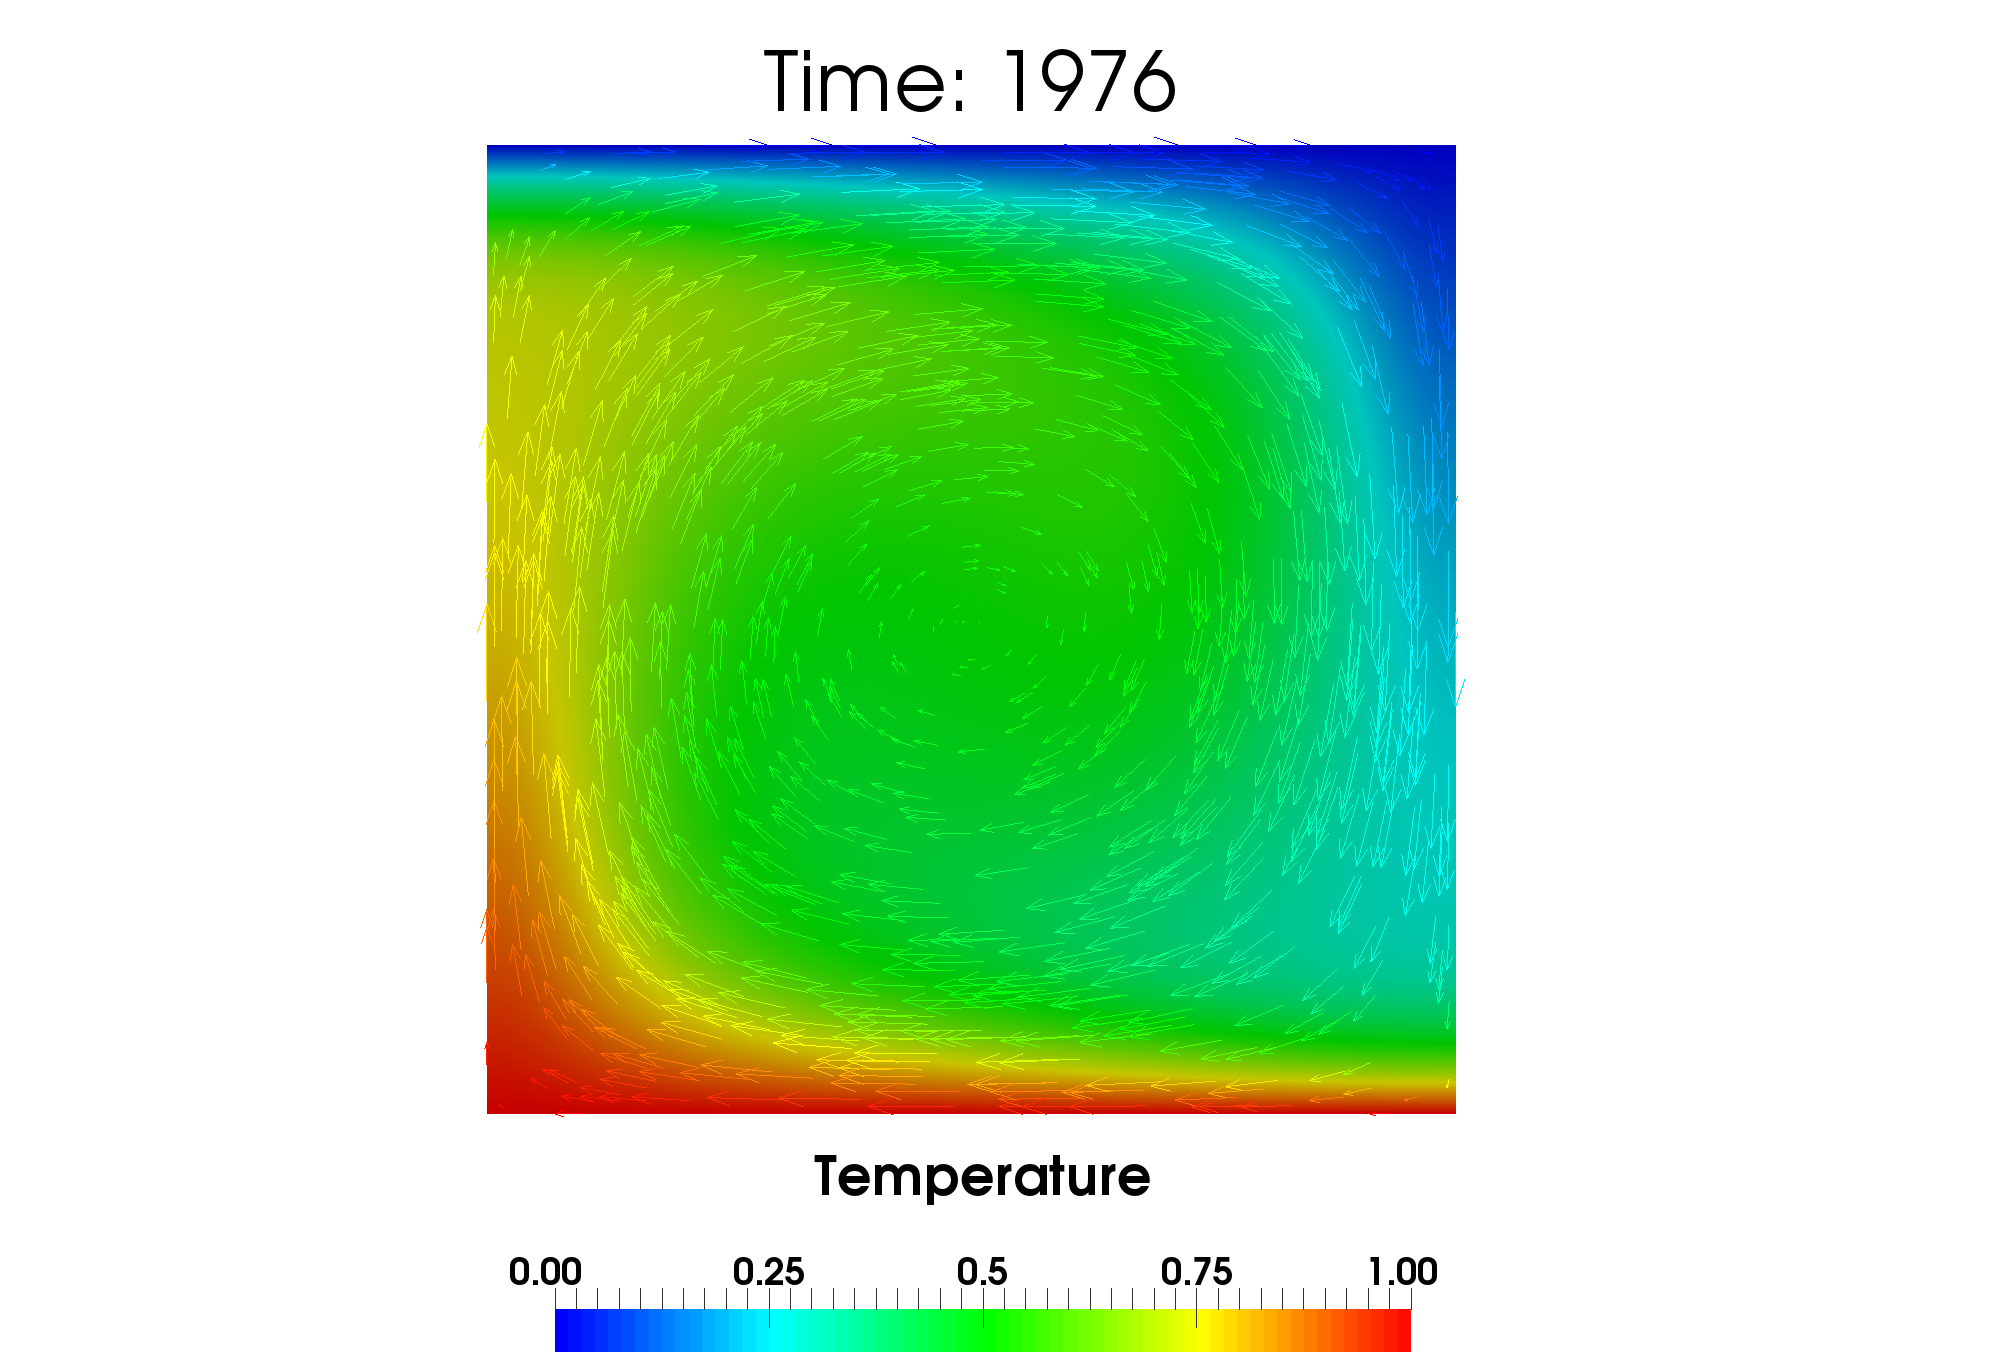
\includegraphics[width=.9\textwidth]{figures/convection_isoviscous_TV.png}
  \caption{Near-steady state solution of a simple isoviscous thermal
    convection problem Blankenbach 1a
    \cite{blankenbach_benchmark_1989} ($\Ra=10^{4}$). Resolution is
    $64\times64\times2$ triangles with mixed element
    $(v,p,T)\in([P2,P2],P1,P2])$ for 54148 total degrees of freedom.  Color field
    shows dimensionless Temperature with the velocity field shown as
    arrows. The steady state stopping criterion for this run was set
    such that all fields change by $\leq10^{-5}$ between time-steps.}
  \label{fig:convection1a}
\end{figure}

\section{Solution using \TF}

To set this problem up in \TF{}, we will reuse a large amount of the
work from our Stoke's MMS solutions but extend it to solve the
time-dependent problem.  The principal changes will be
\begin{itemize}
\setlength{\itemsep}{-.1em}
\item Set the domain to  $[0,1]\times[0,1]$ 
\item Add timestepping options including a simple adaptive time stepper.
\item Adding an additional scalar field $T\in P_{2}$ with initial and
  boundary conditions appropriate  to the system
\item Modifying the non-linear residual to the above UFL
\item Modify the solver to handle an additional field (if using
  fieldsplit block-preconditioners)
\item Adjust appropriate monitors and diagnostics
\end{itemize}

A fully worked out \texttt{tfml} file for this problem using a direct
solver for the full Jacobian (Eq. \ref{eq:4.7}) %along with a script to perform a basic convergence test
can be found in
\texttt{\$TF\_HOME/share/terraferma/tutorials/thermalconvection/ isoviscous/newton\_direct/convection.tfml}.  The
solution is shown in Figure \ref{fig:convection1a}.   




%\pagebreak{}

In more detail, the specific steps required to modify the Stokes mms
problem to solve thermal convection are as follows.
\begin{steps}{Step}
\item Make a new tfml file
  \begin{lstlisting}[style=Bash]
$ mkdir myconvection
$ cd myconvection
$ cp $TF_HOME/share/terraferma/tutorials/stokes/isoviscous/mms/mms_direct/stokes.tfml convection.tfml
$ diamond convection.tfml &
  \end{lstlisting}%$
\item \textbf{Change the geometry:} Under \texttt{geometry->Mesh},
  \begin{steps}{step}

  \item Set rectangle bounds to  $[0,1]\times[0,1]$. 
  \item increase \texttt{number\_cells} to $64\times64$
  \end{steps}
\item \textbf{Change io parameters}
  \begin{steps}{step}
  \item Change \texttt{output\_base\_name} to \texttt{rbconvection}
  \item Change \texttt{visualization->element} to (P2DG)
  \item Add appropriate dump-periods for visualization and statistics
    output.  Under \texttt{dump\_periods} do the following
    \begin{itemize}
    \item Activate \texttt{visualization\_period} and set to
      100. (i.e. output paraview files every 100 dimensionless time units)
    \item Check and output statistics every 5 time steps. Activate
      \texttt{statistics\_period}, change it to
      \texttt{statistics\_period\_in\_timesteps}, and set it to 5
    \item Check for steady state stopping criterion every 10 time
      steps. Activate \texttt{steady\_state\_period} and change it to
      \texttt{steady\_state\_period\_in\_timesteps} and set it to 10
      (i.e. check every 10 time steps  whether the change in the solution from   time-step to time-step is lower than the steady-state tolerance)
    \end{itemize}
  \end{steps}
\item \textbf{Add Time-stepping parameters}:
  \begin{steps}{step}
    \item Activate the \texttt{timestepping} tab and set the following
    \begin{itemize}
    \item \texttt{current\_time} = 0.0
    \item \texttt{finish\_time} = 1.e6
    \end{itemize}
    This will run for a dimensionless time of $10^{6}$ or until the
    solution has approached steady state (see below).
  \item \textbf{Set the time-step coefficient \texttt{dt}} Because we
    include the timestep $\Delta t$ explicitly in the form, we need to
    initialize it as a coefficient.  Unlike other coefficients, we do
    this in the Time-stepping tabs as we can add additional
    constraints such as adaptive time-stepping.
    \begin{itemize}
    \item\textbf{ Set the time-step ufl name.} Unfold\texttt{ coefficient(Timestep)} and set the
      \texttt{ufl\_symbol} to \texttt{dt}
    \item \textbf{Set the initial time-step value.}  The time step is
      of type \texttt{Constant}.  For a constant time-step just unfold the \texttt{type(Constant)} tab all the way to set
      the constant value to a fixed value.  Here however we will use
      adaptive time stepping which allows us to set the initial value
      to \textbf{0.0}. Inspection of Equation (\ref{eq:4.26}) shows that
      for \texttt{dt=0}, the problem reduces to a projection problem
      for $T_{i}$ that will simply set it to the initial condition at
      $t=0$, and then the Stoke's solver will solver for the $\vec{v}$
      and $p$ at the initial time.  After the first time-step, the
      adaptive time stepper will choose an appropriate value of
      \texttt{dt} based on a Courant condition.
    \end{itemize}
  \item \textbf{Set Adaptive Time-stepping parameters}. This problem
    will set a crude adaptive time-stepper based on a Courant number
    constraint.  In general, our constraints will
    scale with $\Delta t$, e.g. the Courant number can be considered a
    field
    \begin{displaymath}
      \alpha = \frac{\Delta t ||\vec{v}||}{h}
    \end{displaymath}
    where $h$ is a measure of the local cell-size.  Given a field
    calculated with the current time-step,  the time-stepper will
    return a modified time-step that keeps $\alpha$ to some maximum
    value (e.g. $\alpha_{max}=1$).  The actual Courant number will be calculated in a
    separate system described below.    Here we just inform TerraFERMA how the
    constraint will be implemented.  Do the following
    \begin{itemize}
    \item Activate the
    \texttt{adaptive} tab and add a \texttt{constraint} named
    \texttt{Courant}.
  \item Add the system name that calculates the constraint set
    \texttt{system = CourantNumber}
  \item Set the field or coefficient that is evaluated
    (i.e. \texttt{Field = CourantNumber}
  \item Set the maximum value of the constraint
    \texttt{requested\_maximum\_value = 2.}
  \item In addition you can set fields to determine how often the
    timestep check is called (\texttt{adapt\_period}) as well as the
    maximum amount of growth per time-step when the time-step is
    increasing.  More details on these parameters is given in the help
    windows in diamond. Here we will just check the time step every
    other step.
  \item Activate and set {adapt\_period\_in\_timesteps = 2}
    \end{itemize}
  \item \textbf{Set a steady state check:} We can also stop the
    time-loop when the change from time-step to time-step for any set
    of monitored fields drops below some tolerance.  To activate a
    steady state check
    \begin{itemize}
    \item Under \texttt{}Activate the \texttt{steady\_state} tab
    \item Set the tolerance to \texttt{1.e-5}
    \end{itemize}
    When we describe the fields below we have the option of adding
    them to the steady-state checker.
  \end{steps}
\item \textbf{Add a few global ufl parameters:}  Sometimes it is
  convenient to define a few ufl parameters that will be included in
  all forms.  Here we will just set the values of $\theta$ and
  $\theta_{v}$ that control the theta weightings for Temperature and
  Velocity and define the viscosity as constant (by putting the
  viscosity here, we can more easily modify it later to non-constant viscosity).  Do the following:
  \begin{itemize}
  \item under \texttt{global\_parameters} activate the \texttt{ufl} tab
  \item replace the (string) with the following ufl
    \begin{lstlisting}[style=UFL]
# theta weightings for Temperature and velocity
theta = 0.5
theta_v = 0.5

# scaled viscosity 
eta = 1.
    \end{lstlisting}

  \end{itemize}
\textbf{Caution:} Global ufl options should be used sparingly
  as any change to them will force a re-compile and a regeneration of
  all the ufl code.  To modify constants as run-time parameters, set
  them up as coefficients.
\item \textbf{Modify System Stokes to System Convection}
  \begin{steps}{step}
  \item \textbf{Change the system name} to  \texttt{Convection} (the \texttt{ufl\_symbol}
    remains the same, \texttt{us})
  \item \textbf{Modify Properties for Velocity}.  We will need two
    sets of boundary conditions to impose the no-flow boundaries (the
    free-stress conditions are imposed in the weak-forms), as well as
    cleaning up some of the diagnostics and setting the steady-state
    checkers.  Do the following
         \begin{steps}{do}
      \item \textbf{Set $v_{x}=0$ on the left and right boundaries}: remove (or
        edit) the existing \texttt{boundary\_condition} tab to have
        the following parameters
        \begin{itemize}
        \item \texttt{boundary\_condition} name=\texttt{LeftRight}
        \item \texttt{boundary\_ids} = 1 2
        \item \texttt{sub\_components} name = \texttt{vx}
        \item \texttt{components} = 0
        \item \texttt{type(Dirichlet)} constant = 0
        \end{itemize}
      \item \textbf{Set $v_{y}=0$ on the top and bottom boundaries}: Repeat (or use the copy paste function in diamond) to
        make a second boundary condition for the top and bottom
        boundaries
        \begin{itemize}
        \item \texttt{boundary\_condition} name=\texttt{TopBottom}
        \item \texttt{boundary\_ids} = 3 4
        \item \texttt{sub\_components} name = \texttt{vy}
        \item \texttt{components} = 1
        \item \texttt{type(Dirichlet)} constant = 0
        \end{itemize}
    \item \textbf{Turn on steady-state checking}: under
      \texttt{diagnostics}, activate the tab
      \texttt{include\_in\_steady\_state} and set the norm to be
      checked to \texttt{linf} (infinity norm)
      \end{steps}
    \item \textbf{Modify Properties for Pressure}
      \begin{itemize}
      \item Move the reference point to $[0.5, 0.5]$
      \item \textbf{Turn on steady-state checking}:  under
      \texttt{diagnostics}, activate the tab
      \texttt{include\_in\_steady\_state} and set the norm to be
      checked to \texttt{linf}
      \end{itemize}
    \item \textbf{Add a new Field and diagnostics for Temperature}.
      Activate a new field and set the following properties, BC's and IC's
      \begin{itemize}
      \item \texttt{name} = \texttt{Temperature}
      \item \texttt{ufl\_symbol (global)} = T
      \item \textbf{Set properties of the \texttt{type(Function)}}
        \begin{steps}{do}
        \item set \texttt{rank(Scalar)}
        \item set \texttt{element(P2)}
        \item set the initial condition
          \begin{displaymath}
            T = 1. - y + 0.2\cos(\pi x)\sin(\pi y)
          \end{displaymath}
using the python Expression
\begin{lstlisting}[style=python]
def val(x):
  from math import sin, cos, pi
  return 1.-x[1] + 0.2*cos(x[0]*pi)*sin(x[1]*pi)
\end{lstlisting}
\item \textbf{Set the Dirichlet boundary condition on the top $T=0$}
  \begin{itemize}
  \item activate a new \texttt{boundary\_condition} tab and name it \texttt{Top}
\item set \texttt{boundary\_ids} = 4
\item set \texttt{sub\_components(All)} $\rightarrow$
  \texttt{type(Dirichlet)}$\rightarrow$ \texttt{constant} =0.0
  \end{itemize}
\item \textbf{Set the Dirichlet boundary condition on the bottom $T=1$}
  \begin{itemize}
  \item activate (or copy) a new \texttt{boundary\_condition} tab and name it \texttt{Bottom}
\item set \texttt{boundary\_ids} = 3
\item set \texttt{sub\_components(All)} $\rightarrow$
  \texttt{type(Dirichlet)}$\rightarrow$ \texttt{constant} =1.0
  \end{itemize}
\item \textbf{Set appropriate Diagnostics for Temperature}:  Here we
  should add to visualization, statistics and steady-state monitoring
  \begin{itemize}
  \item activate \texttt{include\_in\_visualization}
  \item activate \texttt{include\_in\_statistics}. 
\item activate \texttt{include\_in\_steady\_state} and set the norm
  type to \texttt{linf}
  \end{itemize}
        \end{steps}
      \end{itemize}

    \item \textbf{remove the coefficients} for \texttt{AnalyticVelocity},
      \texttt{AnalyticPressure}, and \texttt{src}.
    \item \textbf{Add a new coefficient for the Rayleigh Number}
      \begin{itemize}
      \item set the \texttt{name} = \texttt{RayleighNumber}
      \item set the \texttt{ufl\_symbol (global)} = \texttt{Ra}
      \item set
        \texttt{type(Constant)}$\rightarrow$\texttt{rank(Scalar)}$\rightarrow$\texttt{value(WholeMesh)}$\rightarrow$\texttt{constant}
        = \texttt{1.e4}
      \end{itemize}
    \item \textbf{Update the non-linear solver for convection}
    \begin{steps}{do}
    \item Change the residual from Stokes to full   thermal convection
      by adding the temperature residual i.e. implement the ufl
      described above 
\pagebreak{}
    \begin{lstlisting}[style=UFL]
# theta weighted variables
T_theta = theta*T_i + (1.-theta)*T_n
v_theta = theta_v*v_i + (1.-theta_v)*v_n

# Velocity, Pressure and Temperature residuals
Fv = (inner(sym(grad(v_t)), 2.*eta*sym(grad(v_i))) - 
        div(v_t)*p_i - T_i*v_t[1])*dx
Fp = -p_t*div(v_i)*dx
FT = (T_t*((T_i - T_n) + dt*inner(v_theta, grad(T_theta))) + 
         dt/Ra*inner(grad(T_t), grad(T_theta)))*dx

# Total non-linear residual for the system
F = Fv + Fp + FT
    \end{lstlisting}
  \item \textbf{Change the SNES type to ls}:  This is real newton now
    and you'll need a real non-linear solver.
  \item \textbf{Keep a direct solver for Newton (for the moment)}.  A
    sparse direct solve for the full $3\time3$ block Jacobian is
    inefficient and we will change it shortly to a
    block-preconditioned iterative solver, but for now we'll keep the
    sparse direct solver and use it as a base-line case.
    \end{steps}
  \item \textbf{Use the solver at every time step:} change
    \texttt{solve(at\_start)} to \texttt{solve(in\_timeloop)}
  \item \textbf{Modify/Add some Functionals}
    \begin{itemize}
    \item Remove the functionals \texttt{VelocityL2NormSquared},
      \texttt{VelocityL2NormErrorSquared},
      \texttt{PressureL2NormSquared} and
      \texttt{PressureL2ErrorNormSquared}
    \item \textbf{Add a functional for the Nusselt Number}
      \begin{itemize}
      \item set the \texttt{name = TemperatureNu}
      \item set the \texttt{ufl\_name (functional) = int}
      \item add the ufl
       \begin{lstlisting}[style=UFL]
         int = -T.dx(1)*ds(4)
       \end{lstlisting}
 which will calculate the integral of the heat-flux ($-\nabla T\cdot
 \hat{n}$) across the top boundary.
\end{itemize}
\item \textbf{Add a functional for the rms variation in velocity}
      \begin{itemize}
      \item set the \texttt{name = VelocityvrmsSquared}
      \item set the \texttt{ufl\_name (functional) = int}
      \item add the ufl
       \begin{lstlisting}[style=UFL]
int = Ra*Ra*inner(v,v)*dx
       \end{lstlisting}
 which will calculate the integral of the magnitude squared of the velocity
 field over the domain.  The $\Ra^{2}$ scaling is to make this number
 comparable to the numbers used in \cite{blankenbach_benchmark_1989}.
      \end{itemize}
    \end{itemize}
\end{steps}
  \item \textbf{Add a new system to calculate the Courant Number}.  To
    implement our adaptive time-stepper we need to also calculate a
    field of courant numbers for every cell.
    \begin{steps}{step}
    \item \textbf{Activate a new System} 
      \begin{itemize}
      \item set the \texttt{name = CourantNumber}
      \item choose \texttt{mesh (Mesh)}
      \item set the \texttt{ufl\_name (global) = uc}
      \end{itemize}
    \item \textbf{Activate a new field: CourantNumber} and unfold
     \begin{itemize}
      \item set the \texttt{name = CourantNumber}
      \item set the \texttt{ufl\_name (global) = c}
      \item Under \texttt{type(Function)}
        \begin{itemize}
        \item choose \texttt{rank (Scalar)}
        \item choose \texttt{element (P0)}. We will calculate a
          constant value of $\alpha$ for each cell.
        \item set \texttt{initial\_condition}$\rightarrow$\texttt{constant = 0.}
        \end{itemize}
      \item If you want, \textbf{activate diagnostics} for
        \texttt{include\_in\_visualization}, \texttt{include\_in\_statistics}
      \end{itemize}
      
    \item \textbf{Activate a new Solver}
\begin{itemize}
      \item set the \texttt{name = Solver}
      \item choose \texttt{type (SNES)}
      \item \textbf{set the Residual}
        \begin{itemize}
        \item set the ufl 
\begin{lstlisting}[style=UFL]
# Finite volume style estimate of Courant number
# calculate the outward facing normal component of velocity for each facet
n = FacetNormal(c_e.cell())
vn = dot(v_i, n)
vout = 0.5*(vn + abs(vn))

# project the cell integral of the the outgoing flux from each cell
F = c_t*c_i*dx - 
      c_t('+')*vout('+')*dt('+')*dS - c_t('-')*vout('-')*dt('-')*dS - 
      c_t*vout*dt*ds(1) - c_t*vout*dt*ds(2) - 
      c_t*vout*dt*ds(3) - c_t*vout*dt*ds(4)
    \end{lstlisting}
which is the weak form for $\alpha$ that depends on the timestep
$\Delta t$ and integral of the outgoing flux through each cell. \textbf{CAUTION!}
 if you copy and paste the above UFL from the pdf manual to diamond,
 you will introduce some non-ascii characters into the ufl that will
 break FFC.  In this case,  the single quote character \texttt{'} will need to
 be edited to a standard ascii single quote.
\item set the residual \texttt{ufl\_symbol (solver) = F}
\end{itemize}
\item \textbf{Set the Jacobian}
\begin{itemize}
\item set the ufl 
\begin{lstlisting}[style=UFL]
J = derivative(F,uc_i,uc_a)
    \end{lstlisting}
\item set \texttt{ufl\_symbol (solver) = J}
        \end{itemize}
      \item Set \texttt{relative\_error = 1.e-6}
      \item Set \texttt{max\_iterations = 1}

      \item Set the Linear solver
        \begin{itemize}
        \item Choose \texttt{iterative\_method (preonly)}
        \item Choose \texttt{preconditioner (Jacobi)} (the mass matrix
          for a P0 function is exactly diagonal)
        \end{itemize}
      \item Choose \texttt{solve\_with\_diagnostics} to evaluate the
        courant number only at diagnostics (or whenever the adaptive
        time-stepper is called)
        \end{itemize}

   \end{steps}
  \item \textbf{Test the build using}
   \begin{lstlisting}[style=Bash]
$ tfbuild convection.tfml
$ cd build
$ make -j 3
$ make run
   \end{lstlisting}
or copy the testharness file \texttt{convection.shml} from
\texttt{\$TF\_HOME/tutorials/thermalconvection/isoviscous/newton\_direct}
to your current working directory and run
\begin{lstlisting}[style=Bash]
  $ tfsimulationharness --test convection.shml 
\end{lstlisting}
%$
although you might need to edit it for name consistency.

\end{steps}


%\pagebreak{}
\section{Themes and Variations}

Many of the simple variations demonstrated in Chapter
\ref{cha:stokes-equation} for Stoke's  are readily adapted
to the thermal convection problem.  In particular, we can try many
variations on the fieldsplit block pre-conditioners.

\subsection{Iterative Solvers and Fieldsplit preconditioners}

The previous problem uses a sparse-direct solver on the full
$3\times3$ block Jacobian given by Eq. (\ref{eq:4.7}).  While this is
expected to give optimal convergence of the non-linear problem, these
large coupled systems can be expensive to assemble and solve. However,
\TF{} provides many options for exploring and tuning more efficient
methods that can balance convergence and performance.  For example,we
could also use a physically motivated approximate Jacobian
\begin{equation}
  \label{eq:4.9}
   P = \left[
\begin{array}{ccc}
  K & G  & M \\
  G^{T} & 0 & 0 \\
  0 & 0 & A \\ 
  \end{array}
  \right].
\end{equation}
instead of the full Jacobian $J$. $P$ simply neglects the coupling between temperature and velocity
(by  assuming that $B=0$).  In this case, $P$ is block
upper-triangular such that $P\delta = -\vec{F}$  can be solved
sequentially by first solving for the Temperature correction $\delta
T_{i}$ using
\begin{equation}
  \label{eq:4.14}
  A(\vec{v}_i)\delta T_i = -F_{T}(\vec{u}_i)
\end{equation}
using the previous value for $\vec{v}_i$, then updating the velocity field by solving the linear
Stokes system
\begin{equation}
  \label{eq:4.8}
   \left[
\begin{array}{cc}
  K & G  \\
  G^{T} & 0 \\
  \end{array}
  \right]
  \left[
    \begin{array}{c}
      \vec{\delta v}_i \\
      \delta p_i \\
    \end{array}
  \right] = -\left[
    \begin{array}{c}
      F_{\vec{v}}(\vec{u}_{i}) + M\delta T_{i}\\
      F_p(\vec{u}_{i})\\
    \end{array}
  \right]
\end{equation} .


If we just use $P$ as an approximate Jacobian in a Newton scheme, it
can be shown that if the  viscosity is independent of $T$, this
algorithm is equivalent to a standard Picard splitting which first
solves for the  Temperature field with the current velocity,  then
solves for the velocity with the new temperature,  iterating until
some stopping criteria. However,  if we use $P$ as a
\emph{preconditioner} for solving the exact problem
$J\vec{\delta}=-\vec{F}$ using the full Jacobian,
Eq. (\ref{eq:4.7})  we can  get the expected quadratic
convergence of newton with the computational expense of a Picard
iteration.

Figure \ref{fig:isoviscous_conv_perf} compares the
convergence behavior for four solver strategies 
\begin{description}
\item[newton\_direct]  sparse direct solver on $J$
\item[preonly\_fieldsplit\_direct] Just apply the  preconditioner $P$,
  fieldsplit between $T$ and
  $(\vec{v},p)$ using sparse direct
  solvers on the $A$ and Stokes blocks.  This method is equivalent to solving an approximate Newton
  iteration replacing $J$ with $P$.
\item[newton\_fieldsplit\_direct]  Solve $J\vec{\delta}=-F$ using
  flexible gmres, preconditioned by fieldsplit $P$.
\item[picard\_splitting] Solve two systems sequentially, first solving
  for $T$, then Stokes for $(\vec{v},p)$ and iterating until converged.
\end{description}
All schemes were run until $||F||_{2}<10^{-11}$.  

\begin{figure}[htb]
  \centering
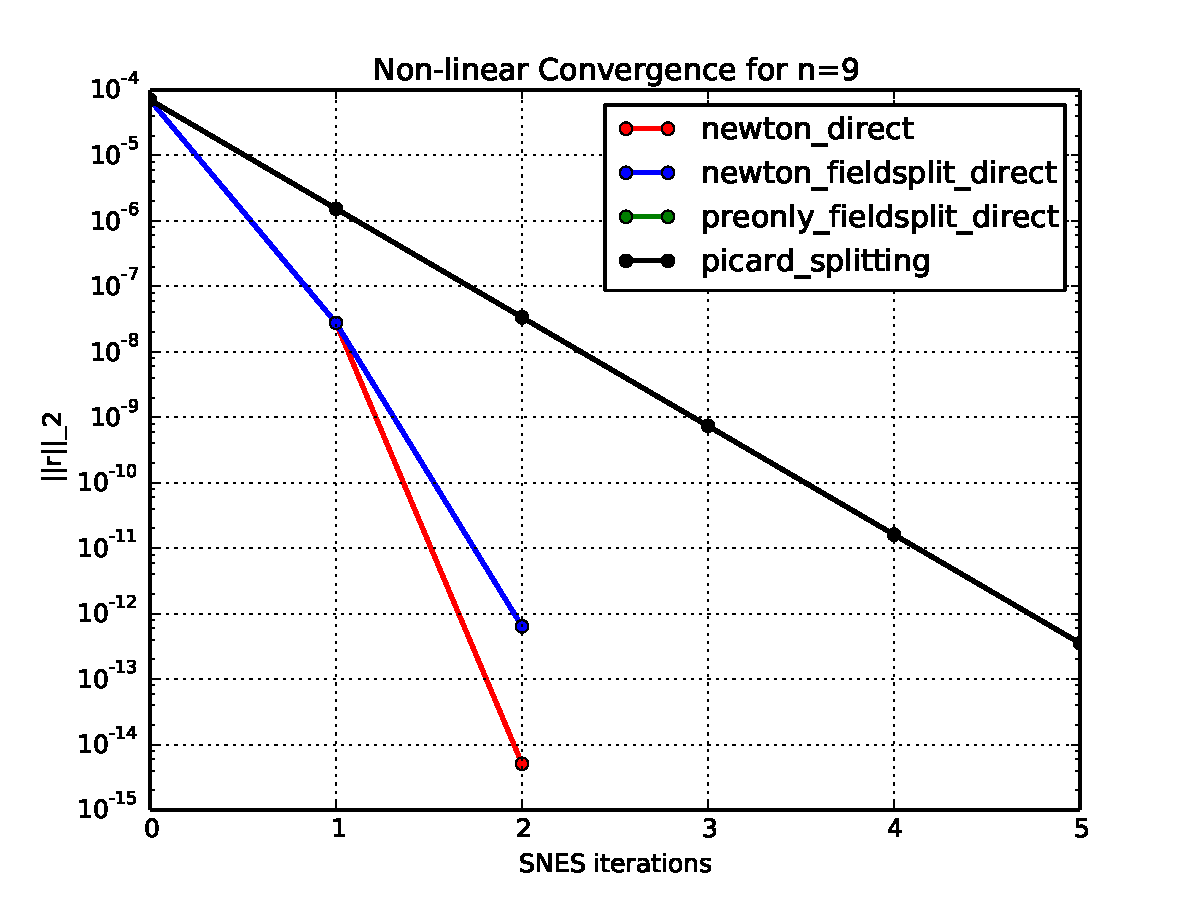
\includegraphics[width=0.5\textwidth]{figures/Solver_comparison_SNES_convergence_isoviscous.pdf}\hfill{}
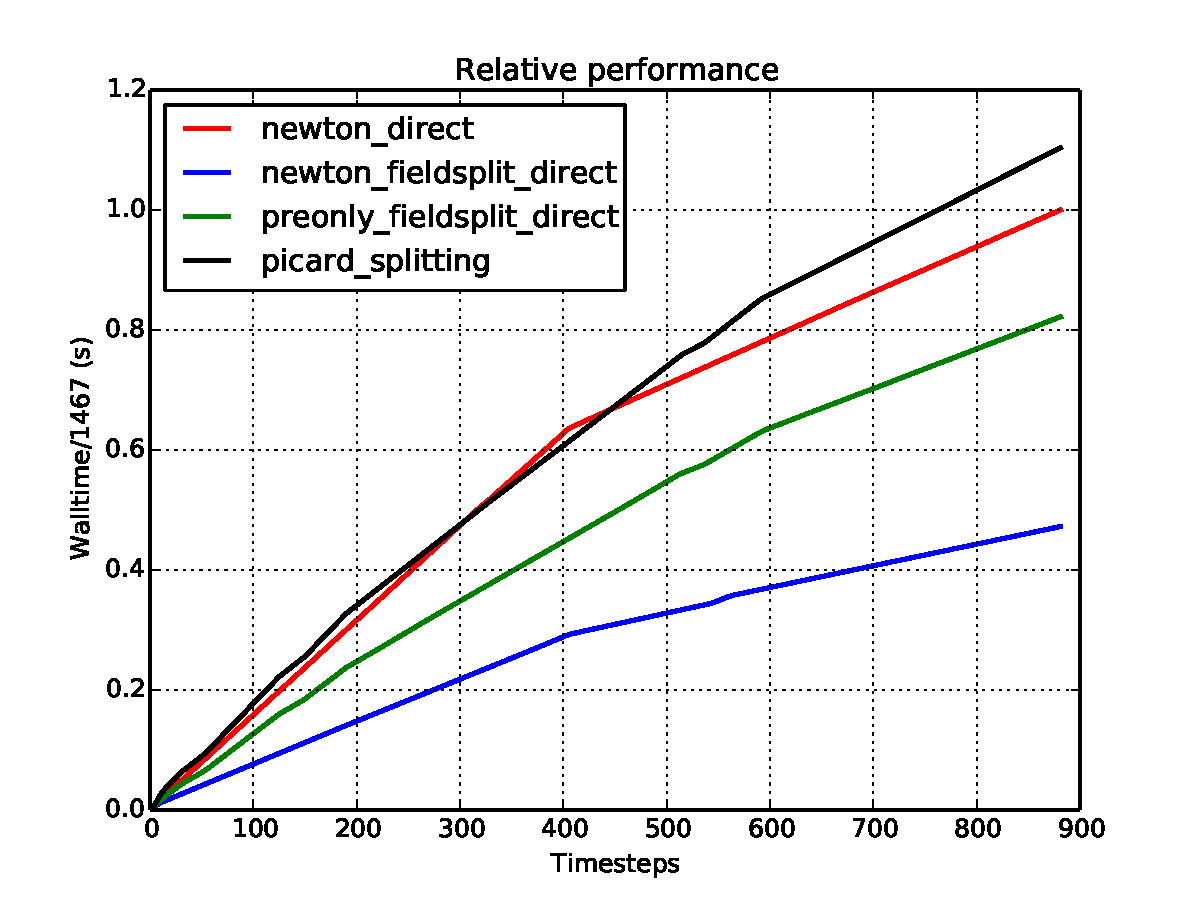
\includegraphics[width=0.5\textwidth]{figures/Solver_comparison_Walltime_isoviscous.pdf}\\
\caption{Comparison of convergence behavior and performance for a
  range of preconditioner-solver options for isoviscous thermal
  convection (Figure \ref{fig:convection1a}).  (\textbf{a})
  convergence behavior of different solver schemes at time-step 9
  showing linear convergence for picard\_splitting and
  preonly\_fieldsplit\_direct (which are identical) and quadratic convergence for
  two Newton schemes   newton\_direct and newton\_fieldsplit\_direct. (\textbf{b}) relative
  performance of the different solver schemes shown as total walltime
  normalized by the maximum time for newton\_direct.  For this problem
the fieldsplit block-preconditioned Newton schemes is $\sim2.5$ times
faster than newton or Picard.}
  \label{fig:isoviscous_conv_perf}
\end{figure}

As expected, Picard splitting and the approximate newton scheme show
the same convergence behavior with $\sim$ 5 non-linear iterations
required for convergence.  Newton\_direct and
newton\_fieldsplit\_direct show quadratic convergence and converge in
2 iterations. 

In terms of performance, however, newton\_direct is more expensive due
to the significantly larger matrix factorization of $J$.  For this
problem, at any rate,  newton\_fieldsplit\_direct is two
times$\sim2.5$ times  faster than both direct Newton and Picard as it has combines the
computational cost of the Picard iteration with much faster
convergence. 


\subsubsection*{Implementation in \TF}
\label{sec:implementation-tf}

Implementing the different solver strategies in \TF{} is relatively
straightforward. Fully worked out examples can be found in the
subdirectories of
\texttt{\$TF\_HOME/share/terraferma/tutorials/thermalconvection/isoviscous}. All
four simulations can be run and Figure \ref{fig:isoviscous_conv_perf}
generated using
\begin{lstlisting}[style=Bash]
  $ tfsimulationharness --test compare_solvers
\end{lstlisting} %$
\textbf{Note}: If you are fortunate to have a multi-core server you
can speed this up significantly by running the four simulations
simultaneously using 
\begin{lstlisting}[style=Bash]
  $ tfsimulationharness --test -n 4 compare_solvers
\end{lstlisting} %$
where \texttt{-n 4} indicates 4 threads.

In more detail, the specific solver setting for the four different
strategies are
\begin{description}
\item[newton\_direct] Under \texttt{nonlinear\_solver
    (Solver)}$\rightarrow$\texttt{type (SNES)}$\rightarrow$\texttt{linear\_solver}
  \begin{itemize}
  \item set \texttt{iterative\_method (preonly)}
  \item set \texttt{preconditioner (lu)} 
  \item choose your favorite
    sparse-direct solver (e.g. \texttt{umfpack} or \texttt{mumps})
  \end{itemize}
\item[preonly\_fieldsplit\_direct] Under \texttt{nonlinear\_solver
    (Solver)}$\rightarrow$\texttt{type (SNES)} $\rightarrow$ \texttt{linear\_solver}
  \begin{itemize}
  \item set \texttt{iterative\_method (preonly)}
  \item set \texttt{preconditioner (fieldsplit)}
    \begin{itemize}
    \item set \texttt{composite\_type (multiplicative)}\footnote{a
        multiplicative fieldsplit preconditioner uses the results of
        previous block solves as they become available.  Thus the
        order of splits is important.  If we solve $T$ then Stokes,
        the preconditioner is upper triangular, otherwise it's lower
        triangular.  A \texttt{composite\_type (additive) is just
          block diagonal}}
    \item Now set the individual fieldsplits and solvers for each
      split.  Here we will have two splits.  The first for Temperature
      $T$, and the second for Stokes $(\vec{v},p)$. We will use sparse
      direct solvers for each of the splits. In detail
      \begin{itemize}
      \item Activate a fieldsplit and set the name to
        \texttt{Temperature}.  Beneath this
        \begin{itemize}
      \item activate a field named
        \texttt{Temperature}
      \item Set the \texttt{linear\_solver} to
        \texttt{iterative\_method (preonly)}  and
        \texttt{preconditioner (lu)}
      \end{itemize}
      \item Activate another fieldsplit and set the name to
        \texttt{Stokes}. Beneath this
        \begin{itemize}
      \item activate a field named  \texttt{Pressure}
      \item activate a field named  \texttt{Velocity}
      \item Set the \texttt{linear\_solver} to
        \texttt{iterative\_method (preonly)}  and
        \texttt{preconditioner (lu)}
      \end{itemize}

      \end{itemize}
    \end{itemize}
  \end{itemize}
\item[newton\_fieldsplit\_direct] Under \texttt{nonlinear\_solver
    (Solver)}$\rightarrow$\texttt{type (SNES)} $\rightarrow$ \texttt{linear\_solver}
  \begin{itemize}
  \item just set \texttt{iterative\_method (fgmres)}
  \item set \texttt{preconditioner (fieldsplit)} and use all the
    fieldsplit options from the previous example.
\end{itemize}
\item[picard\_splitting] \TF{} also allow implementation of more
  classical Picard Splitting schemes for this problem that split the
  problem over two separate systems, one for Temperature, the other
  for Stokes, then solves them sequentially using the output of one
  system as coefficients in the other, but calculating the non-linear
  residual of the entire system $F(T,\vec{v},p)$ at each iteration
  until convergence.  The input file
  \texttt{picard\_splitting/convection.tfml} implements this
  approach.  The key differences that need to be implemented are
  \begin{itemize}
  \item activate \texttt{nonlinear\_systems} (greyed out below
    \texttt{timestepping} options), and set
    \begin{itemize}
    \item \texttt{relative\_error = 1.e-8}
    \item \texttt{absolute\_error = 1.e-11}
    \item \texttt{max\_iterations = 20}
    \item and any monitors of interest
    \end{itemize}
  \item Add or copy a system to just solve Temperature such that
    \begin{itemize}
    \item \texttt{ system name = Temperature}
    \item \texttt{ufl\_symbol (global) = uT}
    \item has a single \texttt{field (Temperature)} with the same BC's
      and IC's as before
    \item Solver settings
      \begin{itemize}
      \item \texttt{Residual}
        \begin{lstlisting}[style=ufl]
T_theta = theta*T_i + (1.-theta)*T_n
v_theta = theta_v*v_i + (1.-theta_v)*v_n

F = (T_t*((T_i - T_n) + dt*inner(v_theta, grad(T_theta))) +
       dt/Ra*inner(grad(T_t), grad(T_theta)))*dx
        \end{lstlisting}
\item \texttt{Jacobian}
        \begin{lstlisting}[style=ufl]
J = derivative(F, uT_i, uT_a)
        \end{lstlisting}
      \end{itemize}
    \item Set linear solver to \texttt{iterative\_method (preonly)},
      \texttt{preconditioner (lu)}
    \item Add any functionals of interest

    \end{itemize}

  \item Add a system to just solve Stokes.
    \begin{itemize}
    \item \texttt{ system name = Convection} (or Stokes?)
    \item \texttt{ufl\_symbol (global) = us}
    \item two fields \texttt{field (Pressure)} and \texttt{field
        (Velocity)} each  with the same BC's
      and IC's as before
    \item Solver settings
      \begin{itemize}
      \item \texttt{Residual}
        \begin{lstlisting}[style=ufl]
Fv = (inner(sym(grad(v_t)), 2.*eta*sym(grad(v_i))) - 
         div(v_t)*p_i - T_i*v_t[1])*dx
Fp = -p_t*div(v_i)*dx

F = Fv + Fp          
        \end{lstlisting}
\item \texttt{Jacobian}
        \begin{lstlisting}[style=ufl]
J = derivative(F, us_i, us_a)
        \end{lstlisting}
      \end{itemize}
    \item Set linear solver to \texttt{iterative\_method (preonly)},
      \texttt{preconditioner (lu)}
    \item Add any functionals of interest
    \end{itemize}
  \end{itemize}
\end{description}




\subsection{Variable Viscosity}
\label{sec:variable-viscosity}

The previous example demonstrates the flexibility of \TF{} to readily
compose and compare different solver strategies.  This ability becomes
even more important for strongly coupled non-linear problems.  For
example, Figure \ref{fig:convectionTVdepVisc} shows a convection
calculation with a more realistic temperature and strain-rate
dependent composite rheology
\begin{equation}
  \label{eq:4.10}
  \eta(T,V) =
  \left[
\frac{1}{\eta_{\text{diff}}} + \frac{1}{\eta_{\text{disl}}} + \frac{1}{\eta_{\text{max}}}
  \right]^{-1}
\end{equation}
where
\begin{align}
  \label{eq:4.11}
  \eta_{diff} = &A_{\text{diff}}\exp
  \left[
\frac{E_{diff}}{RT}
  \right]\\
\eta_{disl} =& A_{\text{disl}}\exp
\left[
\frac{E_{disl}}{nRT}
\right]\tilde{\dot{\epsilon}}_{II}^{1/n -1}\\
\eta_{max} =& 10^{24} ~\mathrm{\,Pa\,\, s}
\end{align}
are appropriate (dimensional) rheologies for diffusion creep,
dislocation creep and a viscosity cap \cite{billen_rheologic_2007}.
These rheologies are readily incorporated directly into the ufl and
are included in all the problems with the
\texttt{global\_parameters}$\rightarrow$\texttt{ufl} field as
\begin{lstlisting}[style=ufl]
# model parameters for determining viscosities
v0    =  Ra*kappa/h             # reference advection velocity m/s
edot0 = (v0/h)                  # scaled strainrate

# definition of strain rate tensor and second invariant
edot = sym(grad(v_i))
eIIreg = sqrt(0.5*(inner(edot,edot) + epssquared))

# dimensional temperature
T0 = 873.00                     # Moho Temperature
delta_T = 1500.00               # temperature difference across system
Tdim = delta_T*T_i + T0          

# inverse  viscosities
A1 = 7573290518.9976 #(eta0/Adiff)
A2 = -26.860705193737846  #-Ediff/R/delta_T
T0p = 873./1500
B1 =  34520.1355950926     # (eta0/Adisl)*(edot0)**inexp
B2 =  -12.37081518517564   # -Edisl/(stressn*R*delta_T)
ietamax = 1.e-5
inv_etadiff = A1*exp(A2/(T_i + T0p))  # scaled inv diffusion creep
inv_etadisl = B1*exp(B2/(T_i + T0p))*(eIIreg**inexp) # scaled inv dislocation creep
# scaled inverse viscosity
inv_etaprime = inv_etadiff + inv_etadisl + ietamax

eta = 1./inv_etaprime
\end{lstlisting}
Here, many of the constant have been hardwired into the ufl, however,
it is generally better to include the constants as coefficients and
control them through the simulation testharness.

In this case the full problem is considerably more non-linear.  In
particular, the Stokes sub-problem is now fully non-linear due to the
dependence of viscosity on the strain-rate tensor through
\begin{equation}
\tilde{\dot{\epsilon}}_{II} = \sqrt{\frac{\dot{\epsilon}(\vec{v}):\dot{\epsilon}(\vec{v}) + \dot{\epsilon}_{\varepsilon}}{2}}
\end{equation}
where we have regularized the second invariant (of the
\emph{dimensionless} velocities) by
$\dot{\epsilon}_{\varepsilon} = 2\times10^{-10}$ to prevent
singularities in the Jacobian at low strain-rates.

The Jacobian matrix, which may again be calculated by automatic differentiation, is still block structured:
\begin{equation}
  \label{eq:TVJacobian}
  J =  \left[
\begin{array}{ccc}
  \left[K + \eta_{\vec{v}}\right] & G  & \left[M + \eta_{T}\right] \\
  G^{T} & 0 & 0 \\
  B & 0 & A \\ 
  \end{array}
  \right]
\end{equation}
but with additional coupling blocks, $\eta_{\vec{v}}(\vec{u}_i)$ and $\eta_{T}(\vec{u}_i)$ due to the variation of viscosity with velocity
and temperature respectively which also make $K(\vec{u}_i)$ non-linear.  
\begin{figure}[htbp!]
  \centering
  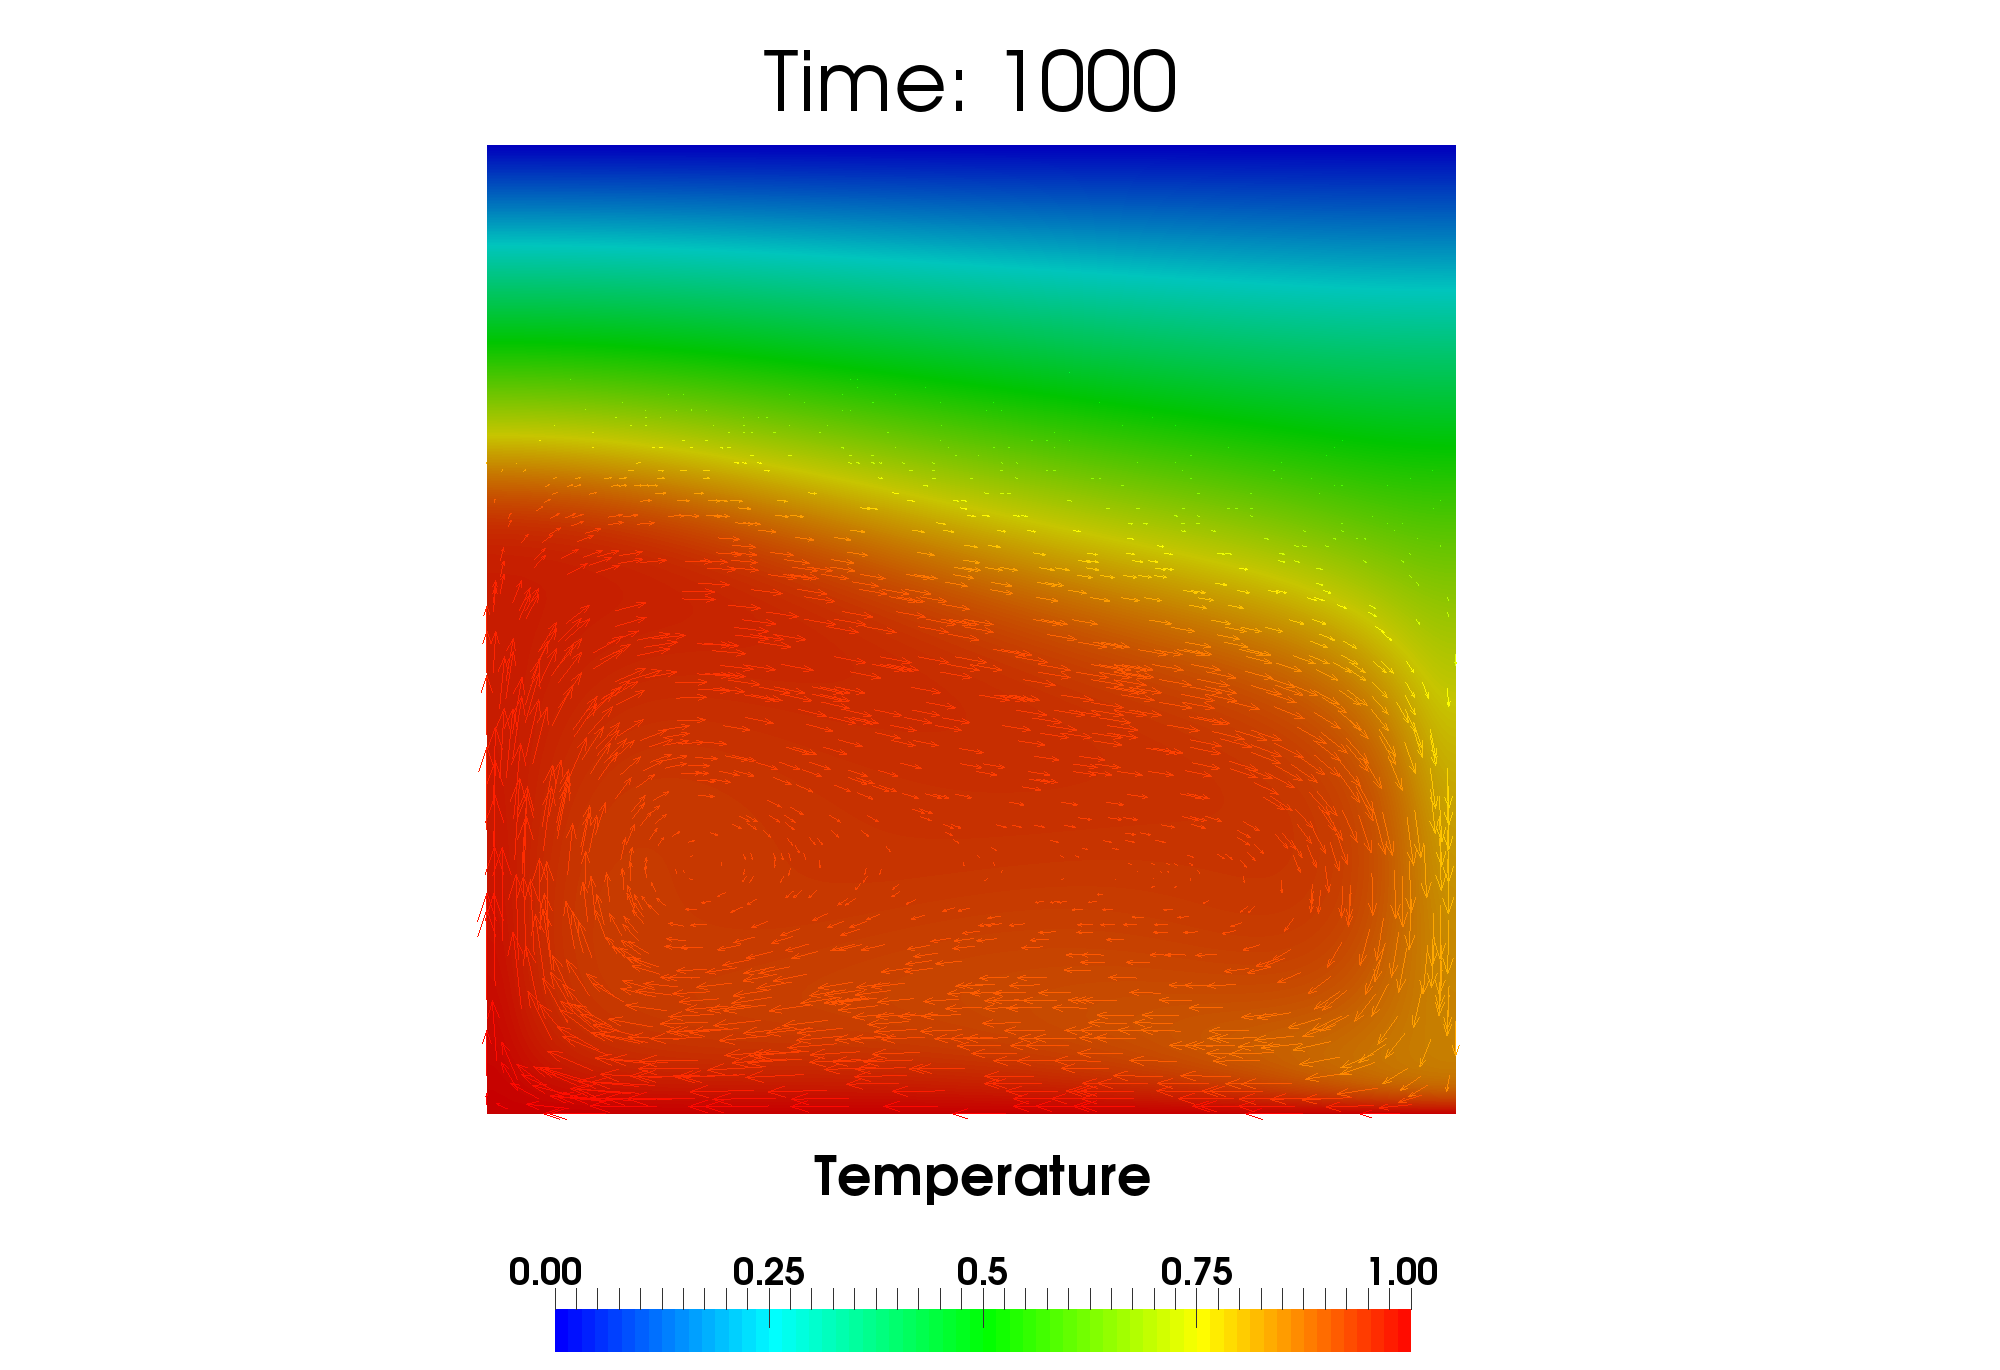
\includegraphics[width=.9\textwidth]{figures/convection_TVdependent_TV.png}
  \caption{Solution of a thermal convection problem with Temperature
    and strainrate dependent viscosity (Eq.~\ref{eq:4.10}) and  nominal Rayleigh Number
    $\Ra=10^{4}$. Numerical parameters and resolution are the same as
    in Figure \ref{fig:convection1a}. Color field shows dimensionless
    Temperature with the velocity field shown as arrows. This model is   described in
    \texttt{\$TF\_HOME/share/terraferma/tutorials/thermalconvection/TVdependentViscosity}
  and demonstrates a stagnant lid and considerably assymetry in flow}
  \label{fig:convectionTVdepVisc}
\end{figure}

\begin{figure}[htb]
  \centering
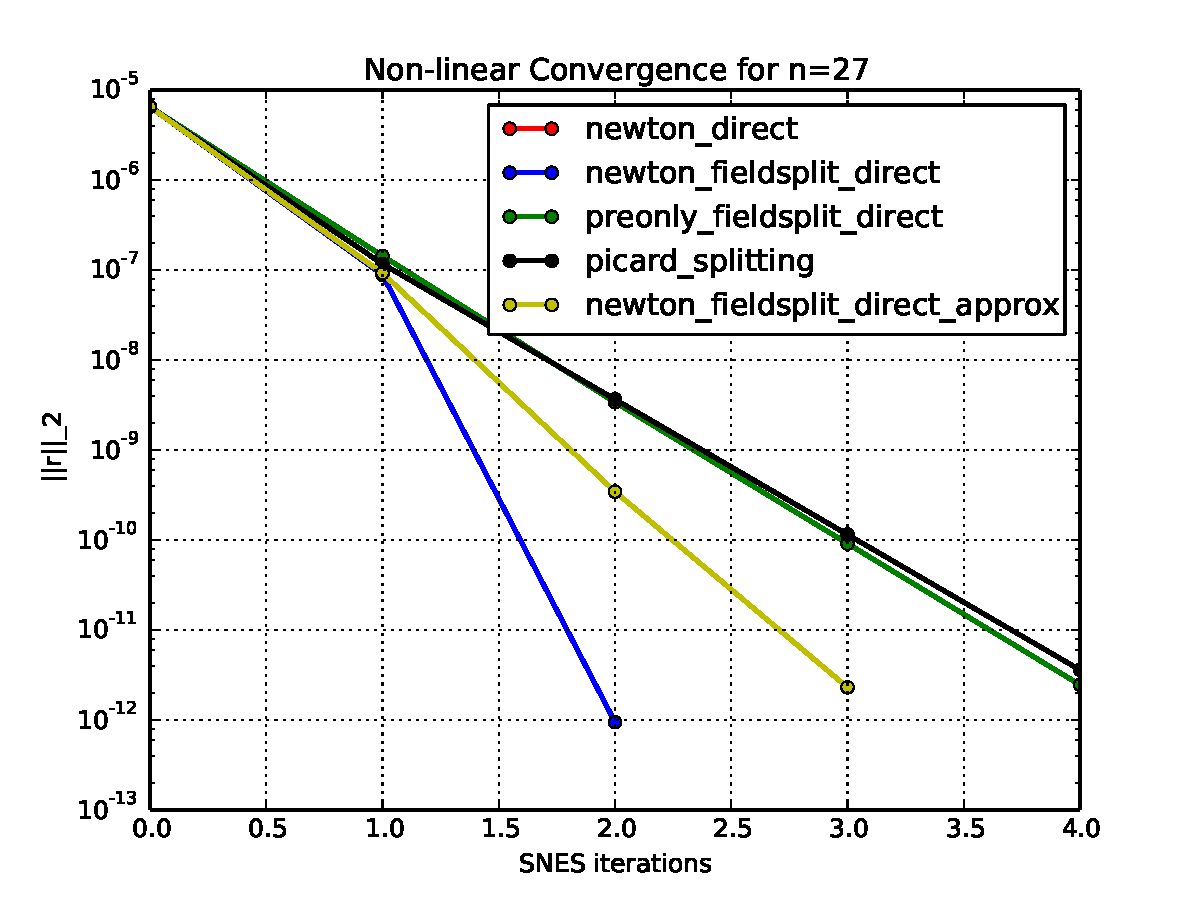
\includegraphics[width=0.49\textwidth]{figures/Solver_comparison_SNES_convergence_TVvisc.pdf}\hfill{}
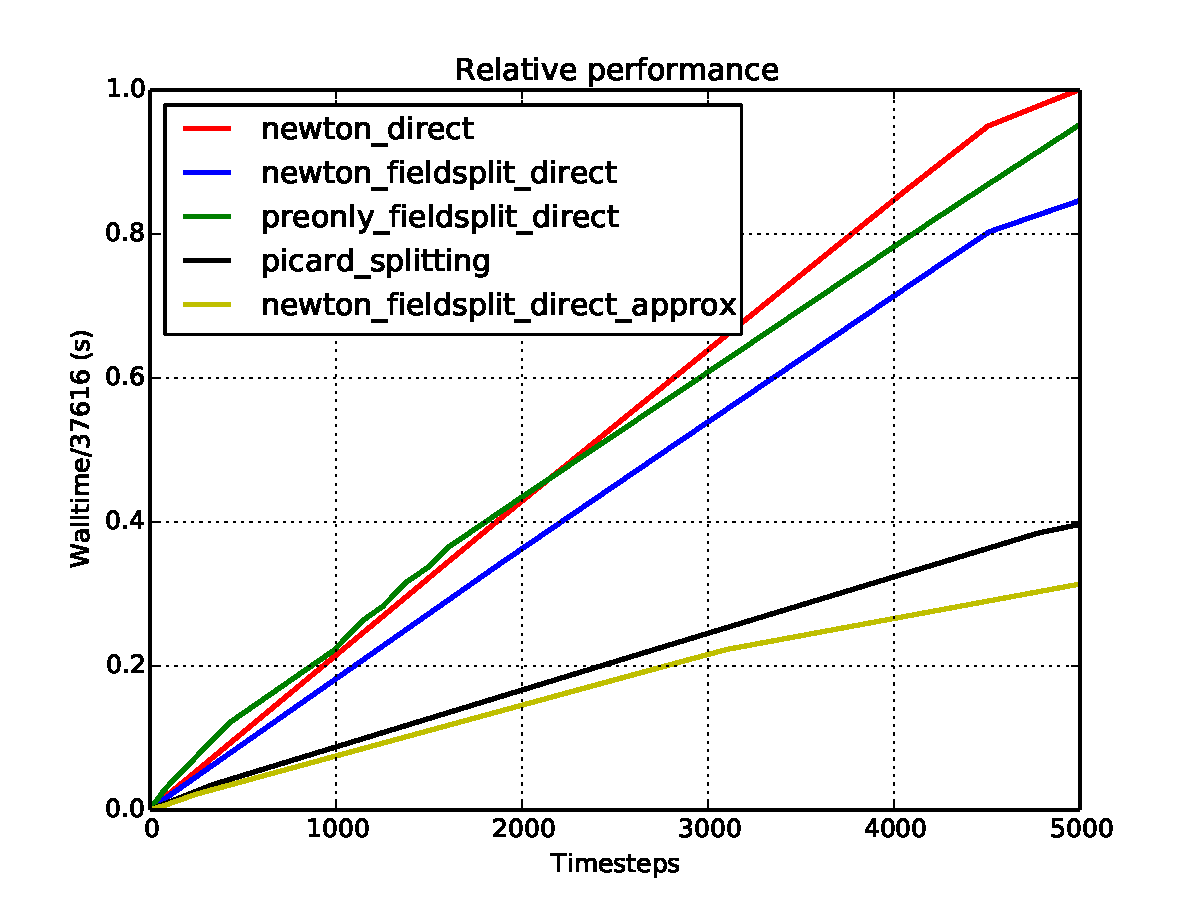
\includegraphics[width=0.49\textwidth]{figures/Solver_comparison_Walltime_TVvisc.pdf}\\
  \caption{Comparison of convergence behavior and performance for a
    range of preconditioner-solver options for  the thermal
    convection problem shown in Figure \ref{fig:convectionTVdepVisc}.  
    (\textbf{a}) convergence behavior of different solver
    schemes at time-step 27 showing linear convergence for
    \texttt{picard\_splitting} and \texttt{preonly\_fieldsplit\_direct}
    and quadratic for \texttt{newton\_direct} and
    \texttt{newton\_fieldsplit\_direct}. An approximate Jacobian shows
    a convergence pattern part-way between linear and quadratic. (\textbf{b}) relative
    performance of different solver schemes normalized by the total
    walltime for \texttt{newton\_direct}. Note: the extra assembly and
    solution    time of the full Jacobian $J$ offsets its gains in
    convergence.  However using an approximate Jacobian that maintains
    the non-linearity in Temperature but not in Velocity performs best
  at near 3 times \texttt{newton\_direct}.  These figures can be
  recreated by running \texttt{tfsimulationharness --test
    compare\_solvers.shml} within the \texttt{TVDependentViscosity} directory.}
  \label{fig:Tvdependentvisc_conv_perf}
\end{figure}

 




Figure \ref{fig:Tvdependentvisc_conv_perf} shows convergence and performance results for the same solver strategies discussed for the
isoviscous case: \texttt{newton\_direct},
\texttt{preonly\_fieldsplit\_direct},
\texttt{newton\_fieldsplit\_direct}, and \texttt{picard\_splitting}
Unlike the isoviscous case, \texttt{preonly\_fieldsplit\_direct} and
\texttt{picard\_splitting} are no longer equivalent. 
% The first
% successively solving
% \begin{equation}
%   \label{eq:TVapproxnewtonsteps}
%   A(\vec{v}_i)\delta T_i = -r_{T}(\vec{u}_i) \quad \textrm{then} \quad
%    \left[
% \begin{array}{cc}
%   \left[K(\vec{u}_i) + K_{\vec{v}}(\vec{u}_i)\right] & G  \\
%   G^{T} & 0 \\
%   \end{array}
%   \right]
%   \left[
%     \begin{array}{c}
%       \vec{\delta v}_i \\
%       \delta p_i \\
%     \end{array}
%   \right] = -\left[
%     \begin{array}{c}
%       r_{\vec{v}}(\vec{u}_i) + \left[M+K_T(\vec{u}_i)\right]\delta T_i\\
%       r_p(\vec{u}_i)\\
%     \end{array}
%   \right]
% \end{equation}
% and the second
% \begin{equation}
%   \label{eq:TVpicardsteps}
%   A(\vec{v}_i)\delta T_i = -r_{T}(\vec{u}_i) \quad \textrm{then} \quad
%    \left[
% \begin{array}{cc}
%   K(\vec{u}_{i+1/2}) & G  \\
%   G^{T} & 0 \\
%   \end{array}
%   \right]
%   \left[
%     \begin{array}{c}
%       \vec{\delta v}_i \\
%       \delta p_i \\
%     \end{array}
%   \right] = -\left[
%     \begin{array}{c}
%       r_{\vec{v}}(\vec{u}_{i+1/2})\\
%       r_p(\vec{u}_{i+1/2})\\
%     \end{array}
%   \right].
% \end{equation}
% Due to the non-linearity of $K(\vec{u}_i)$ and $K_{\vec{v}}(\vec{u}_i)$, $r_{\vec{v}}(\vec{u}_{i+1/2})$ is no longer equivalent to
% $r_{\vec{v}}(\vec{u}_i) + \left[M+K_T(\vec{u}_i)\right]\delta T_i$. 
However, their convergence behaviors are similar with only
marginal gains seen using the approximate Newton scheme.  As before
the full benefits of Newton's method are only seen
using \texttt{newton\_direct} and \texttt{newton\_fieldsplit\_direct},
where the norm of the residual drops $\sim 7$ orders of magnitude in 2
as opposed to 4 iterations.  These higher
convergence rates however come at a higher cost than using
\texttt{picard\_splitting} (see Figure
\ref{fig:Tvdependentvisc_conv_perf}), owing to the increased
computational expense  of assembling and solving the $\eta_{\vec{v}}$
and $\eta_{T}$ blocks in the full Jacobian (Eq.\ \ref{eq:TVJacobian}). 

The above discussion is not intended to be an exhaustive study of
solver strategies for thermal convection, and many more alternatives
are possible.  For example, Figure
\ref{fig:Tvdependentvisc_conv_perf} also shows results for an iterative
Newton scheme, \texttt{newton\_fieldsplit\_direct\_approx} that uses an approximate Jacobian   that maintains the
non-linearity in temperature but does not assemble the
$K_{\vec{v}}$ block in Eq.\ (\ref{eq:TVJacobian}). The only
substantive change from \texttt{newton\_fieldsplit\_direct} is in the
ufl for the residual, which is now
\pagebreak{}
\begin{lstlisting}[style=ufl]
# velocity residual and derivative, viscosity block
rv_v = inner(sym(grad(v_t)), 2.*eta*sym(grad(v_i)))*dx

# remainder of the velocity residual rv = rv_v + rv_r
rv_r =  -(div(v_t)*p_i + T_i*v_t[1])*dx

r_r = rv_r + rp + rT

# approximate Jacobian including derivative of viscosity 
#with respect to T but not V
J = derivative(r_r, us_i, us_a) + 
      inner(sym(grad(v_t)), 2.*eta*sym(grad(v_a)))*dx + 
      derivative(rv_v,(T_i),(T_a))
  
\end{lstlisting}
This scheme has both better convergence and performance than Picard
splitting, \emph{for this particular problem}, where it seems that
most of the solution is actually the diffusion creep regime, so
neglecting the some of the non-linearity due to strain-rate may be an
effective strategy.  More importantly,  these
examples demonstrate, optimal solver strategies can be highly problem
dependent and the flexibility inherent in \TF{} can greatly
facilitate exploring and implementing them.  Again nearly all of this
functionality is inherited from the two core libraries FEniCS and
PETSc, however, \TF{} provides a more uniform and flexible interface
for constructing applications from these libraries.
 


%%% Local Variables: 
%%% mode: latex
%%% TeX-master: "tftutorials"
%%% End: 
